En el plan de la carrera de grado en Ingeniería Mecánica del Departamento de Ingeniería e Investigaciones Tecnológicas (DIIT) de la UNLaM esta asignatura es el nexo entre las primeras propias de la especialidad con las básicas en las que se imparten herramientas de álgebra, análisis matemático, cálculo numérico, y mecánica Newtoniana. El esquema de correlatividades inmediatas a la asignatura Mecánica General, que muestra la figura \ref{fig:correlativas}, deja en claro que esta debe tener entre sus objetivos el mostrar al alumno cómo dichas herramientas tienen aplicación en su tema de interés.

\begin{figure}[!ht]
\centering
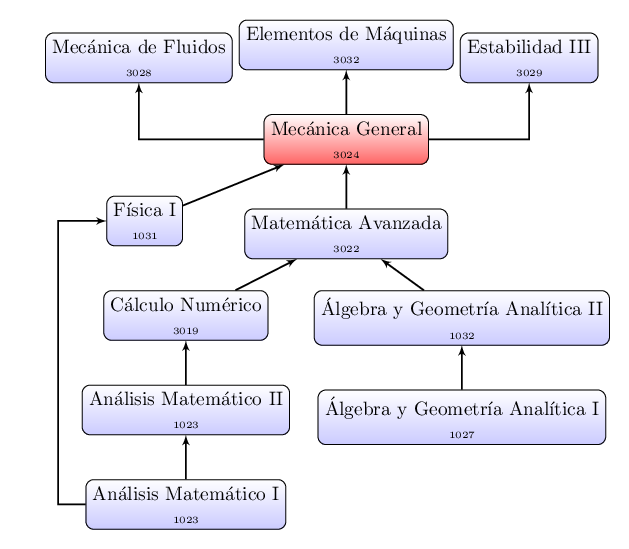
\includegraphics[width=3in]{figuras/correlativas.png}
\caption{Precedida de asignaturas de álgebra, análisis y física, Mecánica General es la primera en que se aplican tales conocimientos a la ingeniería mecánica.}
\label{fig:correlativas}
\end{figure}

La asignatura entrena a los alumnos en la habilidad de modelizar la física de sistemas mecánicos simples. Se entiende por modelizar el realizar una serie de procedimientos con los que se construye un esquema simplificado de la física partiendo de una evaluación semi-cuantitativa de las fuerzas y campos que actúan sobre el sistema así como de las ligaduras que limitan sus grados de libertad. Con tal información se priorizan algunas de estas y se descartan otras para arribar al esquema mencionado. Disponer de tal modelo permite:
\begin{itemize}
    \item elegir coordenadas generalizadas para describir los grados de libertad relevantes,
    \item escribir relaciones matemáticas entre estas que den cuenta de ligaduras,
    \item describir las fuerzas generalizadas que no sean efecto de campos (gravitatorio, electromagnéticos, etc.),
    \item y describir la energía potencial y cinética del sistema en su conjunto.
\end{itemize}

Tras realizar lo anterior se demuestra y se pone en práctica en el curso el formalismo de Euler-Lagrange para obtener un conjunto de ecuaciones diferenciales que describen la dinámica del sistema y/o los esfuerzos mecánicos que cada uno de sus componentes debe soportar en cada instante de tiempo.

De lo expuesto en los párrafos precedentes se evidencia que la temática del curso objeto de este trabajo está circunscrita a la convencional de los cursos de mecánica racional como se detalla en su literatura canónica de referencia \cite{landau}. No es en la temática sino en su metodología didáctica donde se hizo una innovación.

\subsection{El pizarrón, única herramienta didáctica}

Tradicionalmente los sistemas que se trabajan en los cursos de mecánica racional son relativamente simples para acotar el tiempo y/o dificultad de los cálculos de análisis matemático y/o de álgebra que requieren los pasos comentados en el párrafo anterior. Pero esta simplificación extrema lleva a un notorio salto en la complejidad de la que requiere modelar de dispositivos mecánicos, la dinámica de fluidos o a estructuras rígidas, las respectivas temáticas de las asignaturas subsiguientes a Mecánica General (ver figura \ref{fig:correlativas}).

La limitación a la complejidad la impone lo que el docente puede, en la duración de una clase, calcular en el pizarrón. Estos al irse borrando sucesivamente no sólo impide al alumno servirse de referencia de algo que ya no está a la vista sino que además le impone dedicar buena parte de su atención a no cometer errores al transcribir lo allí escrito en su cuaderno. Este soporte en papel a su vez limita la extensión y complejidad de los problemas que pueden proponerse al alumnado para ejercitar lo aprendido. 
Lo  que sintetiza el párrafo precedente no es otra cosa que el proceder en el dictado de clases de ciencias o ingeniería a nivel universitario que se reproduce casi en forma inalterada desde el siglo XIX hasta nuestros días.

\subsection{Herramientas didácticas informáticas}

Los pasos previos y posteriores al obtener un sistema de ecuaciones diferenciales que describen la dinámica y esfuerzos para un modelo mecánico complejo pueden realizarse con herramientas informáticas, pero que son distintas para cada caso.
Para resolver y analizar el resultado de las ecuaciones se aplican las herramientas aprendidas en la asignatura Cálculo Numérico, cursada previamente a Mecánica General, y las ubicuas de graficación para visualizar la evolución temporal de distintas magnitudes. Si bien es cierto que el cálculo numérico se aprovecha ocasionalmente en la ejercitación \cite{mirasso-raichman, caligaris-rodriguez}, este rara vez es utilizado por el docente durante la clase. Se pierde así una oportunidad de ejemplificar mejor y profundizar el análisis del comportamiento de los sistemas modelados.

Pero si es rara la aplicación del cálculo numérico durante las clases lo es aún más el uso de sistemas de álgebra computacional (Computer Algebra Systems o CAS, en inglés), que permiten automatizar todos los procedimientos matemáticos que requiere la modelización: desde definir grados de libertad, sistema de coordenadas, campos y fuerzas externas al modelo hasta construir el sistema de ecuaciones diferenciales para la dinámica. El utilizarlos para resolver cálculos de álgebra lineal y análisis matemático permite quitar el énfasis sobre estos y centrar la atención del docente y alumnos en la temática propia de la asignatura.

Pero la realidad cotidiana de nuestras aulas es que durante las clases dichos cálculos se continúan realizando manualmente en el pizarrón o en papel obviando el uso de la informática. Empeñarse en ese proceder en el nivel universitario sería análogo al de privar al alumnado del uso de calculadoras de bolsillo para realizar procedimientos aritméticos aprendidos en el nivel primario. Todo un anacronismo en la tercera década del siglo XXI.

\subsection{Reciclado del código}

Lo precedente puede interpretarse erróneamente como un mero llamado a utilizar la informática como un análogo de la calculadora de bolsillo, supliendo resultados de los cálculos que demanda la resolución de ejercicios en papel. Eso sería una infrautilización de tal recurso en la clase, repitiendo el patrón que sigue la mayor parte de los usuarios de computadoras que obvian en su uso cotidiano un aspecto fundamental de la informática.

La computadora digital se inventó en la Segunda Guerra Mundial con el fin de realizar cálculos numéricos que se definían manualmente en cada ejecución operando como una calculadora más rápida y con capacidad de automatizar algunos de los procesos de manipulación numérica.  Pero desde la mitad del siglo pasado adquirió la capacidad de operar bajo una serie de instrucciones almacenadas en su memoria sobre cómo procesar información tanto numérica como de otra índole. Tales instrucciones reciben el nombre de programa, y se escriben en un código que respeta la sintaxis de un determinado lenguaje.

Los lenguajes modernos de alto nivel permiten escribir un único código incorporando  todos los procedimientos que requiere la resolución y el análisis de un problema de mecánica racional. Esto abarca desde las aproximaciones asumidas para simplificar la física del mismo hasta el análisis con gráficas de su dinámica y esfuerzos mecánicos pasando por todos los cálculos algebraicos y numéricos intermedios.

Partiendo del objetivo de que los alumnos exploten esta herramienta el curso tuvo por metodología el obviar el trabajo en papel y en su lugar desarrollar la habilidad de escribir en un único código el conjunto de operaciones que requiere la resolución de ejercicios. En clase el docente explicó en forma sincrónica ejemplos de códigos que realizan todos los procedimientos requeridos para modelar un sistema mecánico. En cada clase se provee una guía de ejercicios resolubles haciendo pequeñas modificaciones al código provisto por el docente en esa fecha. Sucesivos ejercicios de complejidad creciente requieren pequeñas modificaciones respecto al código con que se resolvió el anterior. Esta reutilización del código permite un mejor aprovechamiento del tiempo y esfuerzo del alumno que en resoluciones en papel donde debe repetir procedimientos ya realizados en anteriores oportunidades. Clase a clase el alumnado construye una biblioteca de códigos con capacidades crecientes de análisis \cite{Barba2019}.

Hay que aclarar que no se forma al alumno en programación para que cree aplicaciones o algoritmos, lo que se denomina programming en inglés. Lo que se busca es que puedan codificar  (por coding en inglés) las instrucciones para que la computadora realice tareas específicas, en particular cálculos para la ingeniería mecánica.

Algunos alumnos archivan sus resoluciones de ejercicios resueltas en papel como referencia en caso de que se presente una problemática similar más adelante en el cursado de la carrera o en la vida profesional. En los hechos esto rara vez sucede y si recurren en el futuro a algún material relacionado a la asignatura es a su bibliografía, que por lo expuesto anteriormente carece de ejemplos adaptables a modelos más complejos que los comúnmente tratados en la asignatura. Por contrapartida un código es fácilmente aplicable al análisis de una problemática profesional análoga a las vistas en el curso. Al figurar en forma explícita las instrucciones para realizar cada paso del procedimiento es sencillo de revisar, expandir y modificar.